\section{Chamadas Recursivas}

\subsection{Chamadas de funções}

\begin{frame}

    \frametitle{Chamadas de funções}

    \begin{itemize}
        \item No momento em que uma função é {chamada}, algumas 
        {tarefas} são realizadas em plano de fundo para que o programa
        se comporte como esperado
        

        \item Se a função tem {parâmetros}, eles são
        {inicializados} com os valores passados na chamada 
        

        \item O {sistema operacional} tem que saber de onde 
        continuar após o encerramento da função chamada, de modo
        que o ponto de retorno é {armazenado}
        

        \item {Quem chamou} a função tem que ter {acesso} ao 
        retorno da função chamada, logo uma {área de memória} é
        reservada para armazenar este valor

    \end{itemize}

\end{frame}

\begin{frame}
    \frametitle{Chamadas de funções}

    \begin{itemize}
        \item Algumas {informações} devem ser {preservadas} ao        se chamar uma função, para se manter o {estado correto} do
        programa
        

        \item Em relação a função que {realizou} a chamada de um 
        outra função, devem ser preservadas as {variáveis locais} e 
        os seus {parâmetros} 
        

        \item Também deve ser armazenado o {endereço de memória} que 
        aponta para o lugar onde o programa deve {prosseguir} após a         {execução}  da função chamada

    \end{itemize}

\end{frame}

\begin{frame}

    \frametitle{Registro de ativação}

    \begin{itemize}
        \item A área de dados que armazena as informações listadas 
        anteriormente é denominada {registro de ativação} ou
        {\textit{stack frame}}
        

        \item O registro de ativação é alocado {dinamicamente} na 
        {pilha de execução}
        

        \item Este registro {existe} enquanto a função que ele se 
        refere está sendo {executada}

        \item O registro de ativação {guarda} todas as informações 
        necessárias para a correta {execução} e {retorno} de 
        uma função
        

        \item Um registro de ativção é {criado} quando a função é 
        {chamada} e é destruído no {retorno} da função
        

        \item Apenas o registro de ativação da função \code{c}{main()} fica 
        {ativo} durante {toda} a execução do programa

    \end{itemize}

\end{frame}

\begin{frame}[fragile]{Visualização da pilha de execução no início do programa}

    \begin{figure}
        \centering

        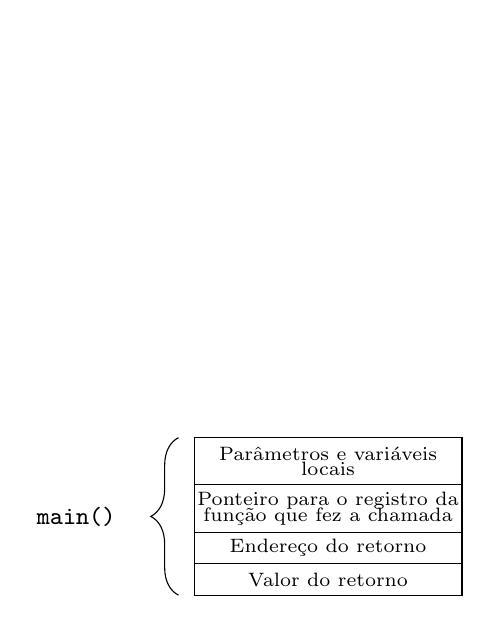
\begin{tikzpicture}
            \draw[opacity=0] (0, 7.2);

            \draw (0, 0) rectangle (3.4, 0.4);
            \draw (0, 0.4) rectangle (3.4, 0.8);
            \draw (0, 0.8) rectangle (3.4, 1.4);
            \draw (0, 1.4) rectangle (3.4, 2.0);

            \node at (1.7, 0.2) { \scriptsize Valor do retorno };
            \node at (1.7, 0.6) { \scriptsize Endereço do retorno };
            \node at (1.7, 1.2) { \scriptsize Ponteiro para o registro da };
            \node at (1.7, 1.0) { \scriptsize função que fez a chamada };
            \node at (1.7, 1.8) { \scriptsize Parâmetros e variáveis };
            \node at (1.7, 1.6) { \scriptsize locais };

            \draw [decorate,decoration={brace, amplitude=10pt}] (-0.2, 0) -- (-0.2, 2);
            \node at (-1.5, 1) { \small \texttt{main()} };

        \end{tikzpicture}

    \end{figure}

\end{frame}

\begin{frame}[fragile]\frametitle{Visualização da pilha após \code{c}{main()} chamar \code{c}{f1()}}

    \begin{figure}
        \centering

        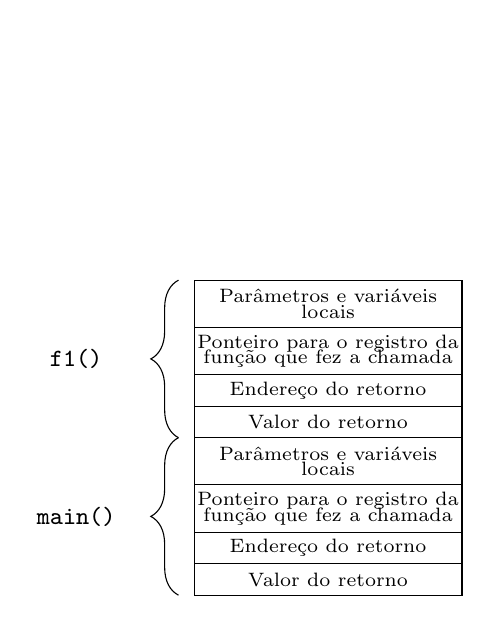
\begin{tikzpicture}
            \draw[opacity=0] (0, 7.2);

            \draw (0, 0) rectangle (3.4, 0.4);
            \draw (0, 0.4) rectangle (3.4, 0.8);
            \draw (0, 0.8) rectangle (3.4, 1.4);
            \draw (0, 1.4) rectangle (3.4, 2.0);

            \node at (1.7, 0.2) { \scriptsize Valor do retorno };
            \node at (1.7, 0.6) { \scriptsize Endereço do retorno };
            \node at (1.7, 1.2) { \scriptsize Ponteiro para o registro da };
            \node at (1.7, 1.0) { \scriptsize função que fez a chamada };
            \node at (1.7, 1.8) { \scriptsize Parâmetros e variáveis };
            \node at (1.7, 1.6) { \scriptsize locais };

            \draw [decorate,decoration={brace, amplitude=10pt}] (-0.2, 0) -- (-0.2, 2);
            \node at (-1.5, 1) { \small \texttt{main()} };

            \draw (0, 2.0) rectangle (3.4, 2.4);
            \draw (0, 2.4) rectangle (3.4, 2.8);
            \draw (0, 2.8) rectangle (3.4, 3.4);
            \draw (0, 3.4) rectangle (3.4, 4.0);

            \node at (1.7, 2.2) { \scriptsize Valor do retorno };
            \node at (1.7, 2.6) { \scriptsize Endereço do retorno };
            \node at (1.7, 3.2) { \scriptsize Ponteiro para o registro da };
            \node at (1.7, 3.0) { \scriptsize função que fez a chamada };
            \node at (1.7, 3.8) { \scriptsize Parâmetros e variáveis };
            \node at (1.7, 3.6) { \scriptsize locais };

            \draw [decorate,decoration={brace, amplitude=10pt}] (-0.2, 2) -- (-0.2, 4);
            \node at (-1.5, 3) { \small \texttt{f1()} };


        \end{tikzpicture}

    \end{figure}

\end{frame}

\begin{frame}[fragile]\frametitle{Visualização da pilha após \code{c}{f1()} chamar \code{c}{f2()}}

    \begin{figure}
        \centering

        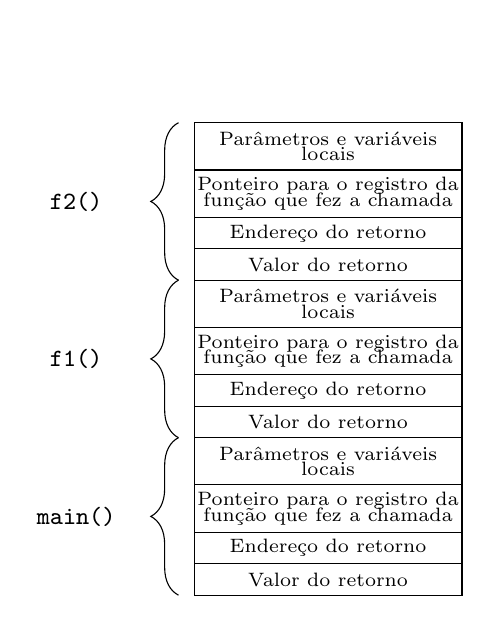
\begin{tikzpicture}
            \draw[opacity=0] (0, 7.2);

            \draw (0, 0) rectangle (3.4, 0.4);
            \draw (0, 0.4) rectangle (3.4, 0.8);
            \draw (0, 0.8) rectangle (3.4, 1.4);
            \draw (0, 1.4) rectangle (3.4, 2.0);

            \node at (1.7, 0.2) { \scriptsize Valor do retorno };
            \node at (1.7, 0.6) { \scriptsize Endereço do retorno };
            \node at (1.7, 1.2) { \scriptsize Ponteiro para o registro da };
            \node at (1.7, 1.0) { \scriptsize função que fez a chamada };
            \node at (1.7, 1.8) { \scriptsize Parâmetros e variáveis };
            \node at (1.7, 1.6) { \scriptsize locais };

            \draw [decorate,decoration={brace, amplitude=10pt}] (-0.2, 0) -- (-0.2, 2);
            \node at (-1.5, 1) { \small \texttt{main()} };

            \draw (0, 2.0) rectangle (3.4, 2.4);
            \draw (0, 2.4) rectangle (3.4, 2.8);
            \draw (0, 2.8) rectangle (3.4, 3.4);
            \draw (0, 3.4) rectangle (3.4, 4.0);

            \node at (1.7, 2.2) { \scriptsize Valor do retorno };
            \node at (1.7, 2.6) { \scriptsize Endereço do retorno };
            \node at (1.7, 3.2) { \scriptsize Ponteiro para o registro da };
            \node at (1.7, 3.0) { \scriptsize função que fez a chamada };
            \node at (1.7, 3.8) { \scriptsize Parâmetros e variáveis };
            \node at (1.7, 3.6) { \scriptsize locais };

            \draw [decorate,decoration={brace, amplitude=10pt}] (-0.2, 2) -- (-0.2, 4);
            \node at (-1.5, 3) { \small \texttt{f1()} };

            \draw (0, 4.0) rectangle (3.4, 4.4);
            \draw (0, 4.4) rectangle (3.4, 4.8);
            \draw (0, 4.8) rectangle (3.4, 5.4);
            \draw (0, 5.4) rectangle (3.4, 6.0);

            \node at (1.7, 4.2) { \scriptsize Valor do retorno };
            \node at (1.7, 4.6) { \scriptsize Endereço do retorno };
            \node at (1.7, 5.2) { \scriptsize Ponteiro para o registro da };
            \node at (1.7, 5.0) { \scriptsize função que fez a chamada };
            \node at (1.7, 5.8) { \scriptsize Parâmetros e variáveis };
            \node at (1.7, 5.6) { \scriptsize locais };

            \draw [decorate,decoration={brace, amplitude=10pt}] (-0.2, 4) -- (-0.2, 6);
            \node at (-1.5, 5) { \small \texttt{f2()} };

        \end{tikzpicture}

    \end{figure}

\end{frame}

\begin{frame}

    \frametitle{Notas sobre os registros de ativação}

    \begin{itemize}
        \item O {endereço de retorno} aponta para o endereço de 
        memória que contém a instrução {imediamente após} a chamada 
        da função
        

        \item O {ponteiro} do registro da função que 
        fez a chamada aponta para o elemento {antecessor}
        da {pilha} de execução
        


        \item Como o {tamanho} dos registros podem variar, o 
        {valor de retorno} fica imediamente acima do registro da 
        função que {fez a chamada}

        \item A criação de {registros de ativação} a cada chamada de 
        função permitem a implementação da {recursão}
        
        \item De fato, a {recursão} consiste em chamar uma função 
        que tem o {mesmo nome} da função que fez a chamada
        
        \item A função não chama a {si mesma}, mas a uma nova 
        instância que tem a {mesma estrutura} da função original

    \end{itemize}

\end{frame}

\begin{frame}[fragile]{Tail Call Optimization}

    \begin{itemize}
        \item \textit{Tail Call Optimization} (TCO) é uma técnica de otimização que permite
            reduzir o espaço utilizado pela pilha de execução

        \item Se o retorno de uma função \code{c}{f()} é a chamada de uma função \code{c}{g()},
            torna-se desnecessário manter o registro de ativação de \code{c}{f()}

        \item Se a função é recursiva e \code{c}{f = g}, então é possível implementar \code{c}{f()} 
            usando espaço em memória constante ($O(1)$)

        \item Se o retorno envolver alguma outra operação que não a chamada de \code{c}{g()}, não 
            será possível usar a TCO
    \end{itemize}

\end{frame}

\begin{frame}[fragile]{Implementação do fatorial que evita a TCO}
    \inputcode{cpp}{fact_no_tco.cpp}
\end{frame}

\begin{frame}[fragile]{Implementação do fatorial que permite a TCO}
    \inputcode{cpp}{fact_tco.cpp}
\end{frame}
